\documentclass[journal,12pt,twocolumn]{IEEEtran}
\usepackage{amsmath,amssymb,amsfonts,amsthm}
\usepackage{txfonts}
\usepackage{tkz-euclide}
\usepackage{listings}
\usepackage{gvv}
\usepackage[latin1]{inputenc}
\usepackage{array}
\usepackage{pgf}
\usepackage{lmodern}

\begin{document}
\bibliographystyle{IEEEtran}

\title{GATE 2023[IN]-36}
\author{EE23BTECH11066 - Yakkala Amarnath Karthik}
\maketitle
\bibliographystyle{IEEEtran}
\textbf{Question:}\\ \\
The impulse response of an LTI system is $h\brak{t}$= $\delta\brak{t}$+0.5$ \delta\brak{t-4}$, where $\delta\brak{t}$ is continuous-time unit impulse signal.if the input signal $x(t)=\cos\brak{\frac{7\pi t}{4}}$,the output is\hfill(GATE IN 2023)\\ \\

\textbf{Solution:}\\
\begin{table}[!h]
  \centering
  \begin{tabular}{|c|c|c|}
    \hline
    \textbf{Variable} & \textbf{Description} & \textbf{value}\\
    \hline
    $\delta\brak{t}$ & continuous-time unit impulse signal & 1 if t=0;\\ & &  0 in other cases\\
   \hline
    $h\brak{t}$ & impulse response & $\delta\brak{t}$+0.5$ \delta\brak{t-4}$ \\
    \hline
    $x\brak{t}$ & input signal  & $x(t)=\cos\brak{\frac{7\pi t}{4}}$ \\
    \hline
    $y\brak{t}$ & output signal & x\brak{t}$ *$ h\brak{t} \\
    \hline
  \end{tabular}
  \caption{A Table with input parameters}
  \label{tab:gate2023in36}
\end{table}\\
 from \tabref{tab:gate2023in36}
\begin{align}
    y\brak{t} &=x\brak{t} * h\brak{t}\\
            &=x\brak{t} * \brak{\delta\brak{t}+0.5 \delta\brak{t-4}}\\
            &=x\brak{t}+0.5x\brak{t-4}\\
            &=\cos\brak{\frac{7\pi t}{4}}+0.5\cos\brak{\frac{7\pi \brak{t-4}}{4}}\\
            &=\cos\brak{\frac{7\pi t}{4}}+0.5\cos\brak{\frac{7\pi t}{4}-7\pi}\\
            &=0.5\cos\brak{\frac{7\pi t}{4}}
\end{align}

  \begin{figure}[ht]
        \centering
        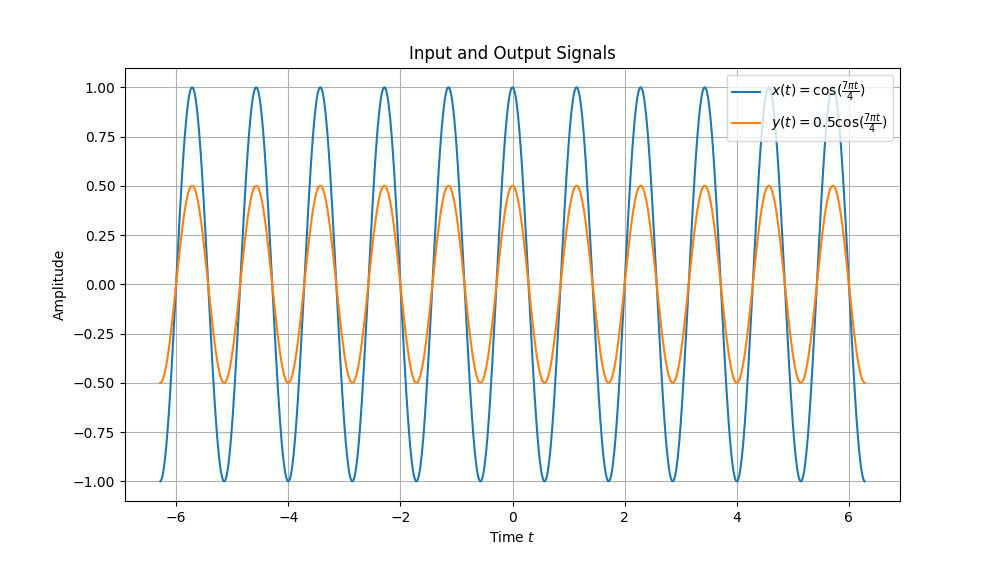
\includegraphics[width=0.45\textwidth]{figs/pythongate.png}
        \caption{Graph showing first 8 terms of the GP}
    \end{figure} 

\end{document}
